\subsection*{Aufgabe 15}
Gegeben ist die Dispersionsrelation für Elektronen in einem fcc-Gitter:
\begin{align*}
  E_{h_1, h_2, h_3}(\vec k) &= \frac{\hbar^2}{2 m_e}(\vec k + \vec G_{h_1, h_2, h_3})^2
  \quad \text{mit}\; \vec G_{h_1, h_2, h_3} = \frac{2 \pi}{a}
  \begin{pmatrix} - h_1 + h_2 + h_3 \\  + h_1 - h_2 + h_3  \\ + h_1 + h_2 - h_3 \end{pmatrix}
  \,;\quad h_i \in \ZZ
\end{align*}
Entsprechend der Empfehlung im Skript führen wir reduzierte Größen $\epsilon$ und
$\vec \kappa$ ein:
\begin{align}
\nonumber
&\vec \kappa := \vec k \cdot \left(\frac{2 \pi}{a}\right)^{-1} \,;\quad
  \epsilon(\vec \kappa) := \frac{E(\vec k)}{E_0}  \,;\quad
  E_0 = \frac{\hbar^2}{2 m_e} \left(\frac{2 \pi}{a}\right)^2
\intertext{Damit wird die Dispersionsrelation}
\label{eq-disp1}
&\epsilon_{h_1, h_2, h_3}(\vec k) = (\kappa_x-h_1+h_2+h_3 )^2 +
   (\kappa_y+h_1-h_2+h_3 )^2 + (\kappa_z+h_1+h_2-h_3 )^2
\end{align}

\subsubsection*{a)}
Im reziproken Gitter liegt der $\Gamma$-Punkt im Ursprung, die Brillouin-Zone
in [111]-Richtung (Raumdiagonale) erstreckt sich bis zum L-Punkt mit den
Koordinaten $\frac{1}{2} (\vec b_1 + \vec b_2 + \vec b_3)$. In [111]-Richtung
gilt also stets $k_x = k_y = k_z$ bzw. $\kappa_x = \kappa_y = \kappa_z =: x$
mit möglichen $x$-Werten zwischen 0 und $\frac{1}{2}$.
Damit wird die Dispersionsrelation \eqref{eq-disp1}:
\begin{align}
\nonumber
\epsilon_{h_1, h_2, h_3}(x) &= (x-h_1+h_2+h_3 )^2 + (x+h_1-h_2+h_3 )^2 + (x+h_1+h_2-h_3 )^2 \\
\label{eq-disp2}
& = 3 x^2 + 2 x (h_1+h_2+h_3) -2 (h_1 h_2 + h_2 h_3 + h_3 h_1) + 3 (h_1^2 + h_2^2 + h_3^2)\\
\label{eq-disp3}
& = a x^2 + b x + c;
\end{align}
Für das unterste Band ($n = 1$) ist $h_1 =  h_2 =  h_3 = 0$, damit wird:
\begin{align*}
  \epsilon_{000}(x) = 3 x^2 \,;\quad
  \epsilon_{000}(L) = \epsilon_{000}\left(\frac{1}{2}\right) = \frac{3}{4} \,;\quad
  E_{000}(L) = E_0 \cdot \epsilon_{000}(L) = \frac{3 \hbar^2}{2 m_e} \left(\frac{\pi}{a}\right)^2
\end{align*}
Für die höheren Dispersionszweige haben wir mit einer Tabellenkalkulation alle
$h_i \in \{-1, 0, 1\}$ variiert (27 Kombinationen) jeweils $a, b, c$ gemäß Formel
\eqref{eq-disp2} und \eqref{eq-disp3} ausgewertet, siehe Tabelle \ref{tab1}.
Die Bänder wurden entsprechend dem Wert $\epsilon(0,5)$ und anschließend nach
$\epsilon(0)$ als Bandnummer $n$ sortiert. Aus der Tabelle ist auch der
Entartungsgrad ersichtlich (= 1, 1, 3, 3).
\begin{table}[!ht]
\caption{Teil a) Dispersionszweige und Entartungsgrad}
\begin{center}
\begin{tabular}{|c|c|c|c|c|c|r|r|c|}
\hline
\textbf{h1} & \textbf{h2} & \textbf{h3} & \textbf{a} & \textbf{b} & \textbf{c}
& \multicolumn{1}{c|}{\textbf{e(0)}} & \multicolumn{1}{c|}{\textbf{e(0,5)}} & \textbf{n} \\ \hline
0 & 0 & 0 & 3 & 0 & 0 & 0,00 & 0,75 & 1 \\ \hline
-1 & -1 & -1 & 3 & -6 & 3 & 3,00 & 0,75 & 2 \\ \hline
-1 & 0 & 0 & 3 & -2 & 3 & 3,00 & 2,75 & \multicolumn{ 1}{c|}{3} \\ \cline{ 1- 8}
0 & -1 & 0 & 3 & -2 & 3 & 3,00 & 2,75 & \multicolumn{ 1}{c|}{} \\ \cline{ 1- 8}
0 & 0 & -1 & 3 & -2 & 3 & 3,00 & 2,75 & \multicolumn{ 1}{c|}{} \\ \hline
-1 & -1 & 0 & 3 & -4 & 4 & 4,00 & 2,75 & \multicolumn{ 1}{c|}{4} \\ \cline{ 1- 8}
-1 & 0 & -1 & 3 & -4 & 4 & 4,00 & 2,75 & \multicolumn{ 1}{c|}{} \\ \cline{ 1- 8}
0 & -1 & -1 & 3 & -4 & 4 & 4,00 & 2,75 & \multicolumn{ 1}{c|}{} \\ \hline
0 & 0 & 1 & 3 & 2 & 3 & 3,00 & 4,75 & \multicolumn{ 1}{c|}{5} \\ \cline{ 1- 8}
0 & 1 & 0 & 3 & 2 & 3 & 3,00 & 4,75 & \multicolumn{ 1}{c|}{} \\ \cline{ 1- 8}
1 & 0 & 0 & 3 & 2 & 3 & 3,00 & 4,75 & \multicolumn{ 1}{c|}{} \\ \hline
1 & 1 & 1 & 3 & 6 & 3 & 3,00 & 6,75 & 6 \\ \hline
0 & 1 & 1 & 3 & 4 & 4 & 4,00 & 6,75 & \multicolumn{ 1}{c|}{7} \\ \cline{ 1- 8}
1 & 0 & 1 & 3 & 4 & 4 & 4,00 & 6,75 & \multicolumn{ 1}{c|}{} \\ \cline{ 1- 8}
1 & 1 & 0 & 3 & 4 & 4 & 4,00 & 6,75 & \multicolumn{ 1}{c|}{} \\ \hline
-1 & 0 & 1 & 3 & 0 & 8 & 8,00 & 8,75 & \multicolumn{ 1}{c|}{8} \\ \cline{ 1- 8}
-1 & 1 & 0 & 3 & 0 & 8 & 8,00 & 8,75 & \multicolumn{ 1}{c|}{} \\ \cline{ 1- 8}
0 & -1 & 1 & 3 & 0 & 8 & 8,00 & 8,75 & \multicolumn{ 1}{c|}{} \\ \cline{ 1- 8}
0 & 1 & -1 & 3 & 0 & 8 & 8,00 & 8,75 & \multicolumn{ 1}{c|}{} \\ \cline{ 1- 8}
1 & -1 & 0 & 3 & 0 & 8 & 8,00 & 8,75 & \multicolumn{ 1}{c|}{} \\ \cline{ 1- 8}
1 & 0 & -1 & 3 & 0 & 8 & 8,00 & 8,75 & \multicolumn{ 1}{c|}{} \\ \hline
-1 & -1 & 1 & 3 & -2 & 11 & 11,00 & 10,75 & \multicolumn{ 1}{c|}{9} \\ \cline{ 1- 8}
-1 & 1 & -1 & 3 & -2 & 11 & 11,00 & 10,75 & \multicolumn{ 1}{c|}{} \\ \cline{ 1- 8}
1 & -1 & -1 & 3 & -2 & 11 & 11,00 & 10,75 & \multicolumn{ 1}{c|}{} \\ \hline
-1 & 1 & 1 & 3 & 2 & 11 & 11,00 & 12,75 & \multicolumn{ 1}{c|}{10} \\ \cline{ 1- 8}
1 & -1 & 1 & 3 & 2 & 11 & 11,00 & 12,75 & \multicolumn{ 1}{c|}{} \\ \cline{ 1- 8}
1 & 1 & -1 & 3 & 2 & 11 & 11,00 & 12,75 & \multicolumn{ 1}{c|}{} \\ \hline
\end{tabular}
\end{center}
\label{tab1}
\end{table}
Die 4 untersten Bänder sind somit:
\begin{align*}
n = 1:\quad & \epsilon_{000}(x) = 3 x^2 \\
n = 2:\quad & \epsilon_{\bar1\bar1\bar1}(x) =  3 x^2 - 6 x + 3\\
n = 3:\quad & \epsilon_{\bar100}(x) = \epsilon_{0\bar10}(x) = \epsilon_{00\bar1}(x) =  3 x^2  - 2 x + 3\\
n = 4:\quad & \epsilon_{\bar1\bar10}(x) = \epsilon_{\bar10\bar1}(x) = \epsilon_{0\bar1\bar1}(x) = 3 x^2 - 4 x + 4\\
\end{align*}
\suppressfloats

\begin{wrapfigure}{R}{12cm}
  \centering
  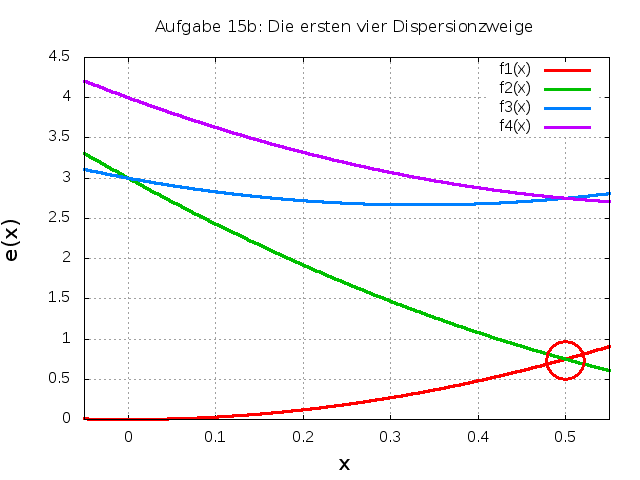
\includegraphics[width=8cm]{aufgabe15b.png}
\caption{zu Aufgabe 15 b)}
\end{wrapfigure}
\subsubsection*{b)}
Überschneidungen gibt es zwischen der 1. und 2. Kurve bei $x = 0,5$, zwischen der
2. und 3. Kurve bei $x = 0$ und zwischen der 3. und 4. Kurve bei $x = 0,5$.
An diesen Stellen erwarten wir Aufspaltungen der Bänder.
\newpage


\subsubsection*{c)}

\subsubsection*{d)}

